\documentclass[12pt]{article}
 
\usepackage[margin=1in]{geometry} 
\usepackage{amsmath,amsthm,amssymb}
\usepackage{graphicx}
\usepackage{epstopdf}
 
\newcommand{\N}{\mathbb{N}}
\newcommand{\Z}{\mathbb{Z}}
 
\newenvironment{exercise}[2][Exercise]{\begin{trivlist}
\item[\hskip \labelsep {\bfseries #1}\hskip \labelsep {\bfseries #2.}]}{\end{trivlist}}
\newenvironment{problem}[2][Problem]{\begin{trivlist}
\item[\hskip \labelsep {\bfseries #1}\hskip \labelsep {\bfseries #2.}]}{\end{trivlist}}
\usepackage{pdfpages}                    			    % Einbindung von PDF-Seiten
\usepackage{geometry}
\usepackage{courier}
\usepackage{color}
\usepackage{listings}
\definecolor{dkgreen}{rgb}{0,0.6,0}
\definecolor{gray}{rgb}{0.5,0.5,0.5}
\definecolor{ghostwhite}{rgb}{0.97, 0.97, 1.0}
\definecolor{vividviolet}{rgb}{0.62, 0.0, 1.0}

\lstset{language=Matlab,
   keywords={break,case,catch,continue,else,elseif,end,for,function,
      global,if,otherwise,persistent,return,switch,try,while},
   basicstyle=\ttfamily,
   keywordstyle=\color{blue},
   commentstyle=\color{dkgreen},
   stringstyle=\color{vividviolet},
   numbers=left,
   numberstyle=\tiny\color{gray},
   stepnumber=1,
   numbersep=10pt,
   backgroundcolor=\color{ghostwhite},
   tabsize=2,
   showspaces=false,
   showstringspaces=false}
   
   
%%%%CHanges von Julian
\usepackage{xcolor}
\usepackage{changebar} 

\newcommand{\removed}[1]{\cbstart\removedfragile{#1}\cbend{}}
\newcommand{\removedfragile}[1]{{\color{red}{#1}}{}} 
\newcommand{\added}[1]{
		{#1}
	%	{\cbstart\addedfragile{#1}\cbend{}}
} 
\newcommand{\addedfragile}[1]{{\color{green!50!black}{#1}}{}} 
\newcommand{\changed}[2]{
		{#1}
	%	{\added{#1}\removed{#2}}
} 



%%%%   
   

\begin{document}
 
% --------------------------------------------------------------
%                         Start here
% --------------------------------------------------------------
 
\title{Weekly Homework 3}
\author{Benjamin Cramer, Julian G\"oltz\\
Brain Inspired Computing}
 
\maketitle
 
\begin{exercise}{3.1}
Stability Conditions in 2D \\
\renewcommand{\labelenumi}{\alph{enumi})}
\begin{enumerate}
\item Requirement for stability $r_\pm < 0$ \changed{with}{wit} $\lambda_\pm = r \pm \added{i} \omega$; eigenvalues given by:
	\begin{equation}
		\lambda_\pm = \frac{1}{2}\left( F_u + G_w \pm \sqrt{(F_u + G_w)^2 - 4(F_uG_w - F_w G_u)}\right)
	\end{equation}
	if $\sqrt{\cdots}$ gets imaginary $\Rightarrow$ $r_\pm <0$ since $F_u+G_w < 0$ \added{(Condition 1)}
	if $\sqrt{\cdots}$ gets real:
	\begin{equation}
		\sqrt{(F_u + G_w)^2 - 4(F_uG_w - F_w G_u)} < \sqrt{(F_u + G_w)^2} = |F_u + G_w|
	\end{equation}
	where we used condition number two; plugging this into eigenvalue expression leads us to:
	\begin{equation}
		\lambda_\pm \leq \frac{1}{2}(F_u + G_w \pm |F_u + G_w|) \leq 0
	\end{equation}
	in both cases the system is stable since $r_\pm < 0$
\item Using the following Mathematica code to obtain fixed points and decide whether they are stable:

	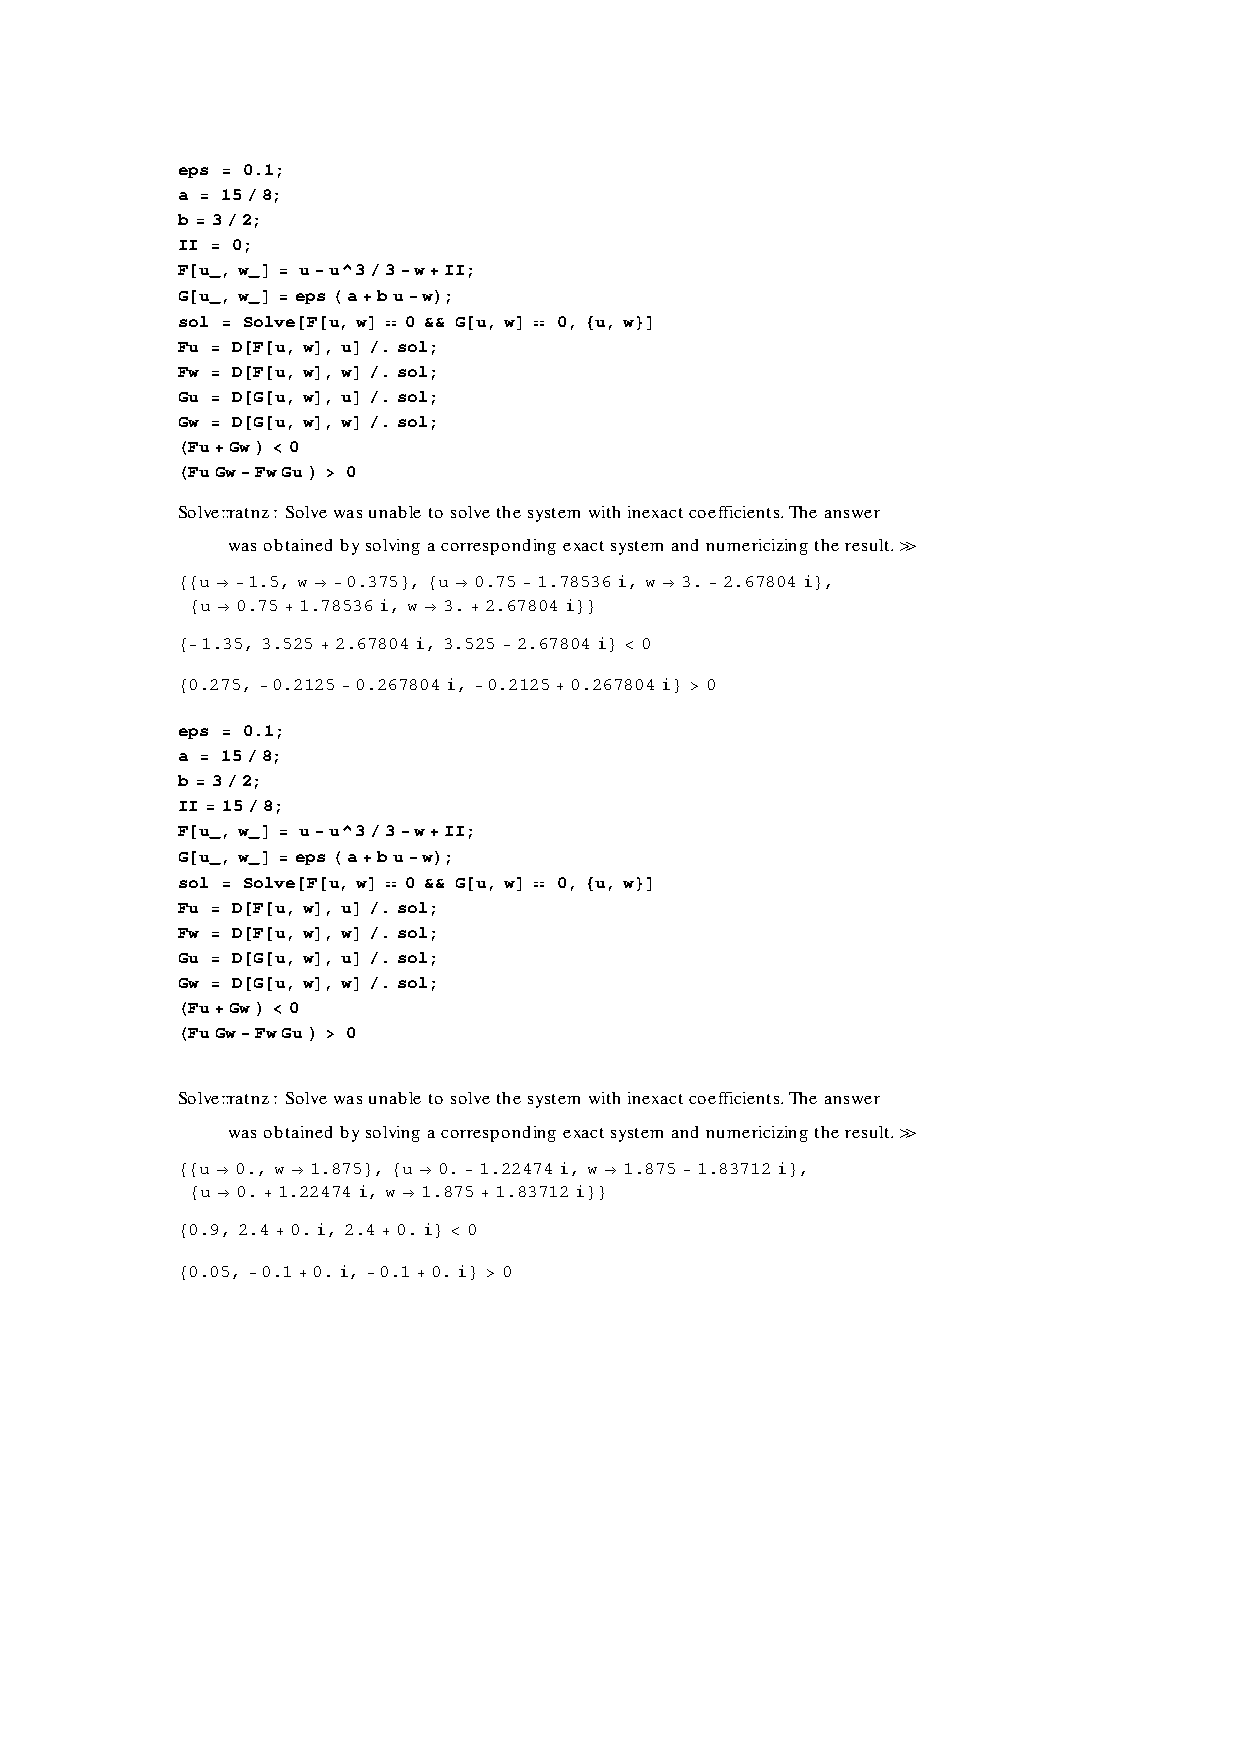
\includegraphics[width=6.5in]{excercise_31}
	\added{From this we follow that for $I=0$ there exists a stable FP (the first result: at $u= -1.5$ and $w=-0.375$, these values are used as initial values below). For the other case there is no FP.}
\end{enumerate}

\end{exercise}

\begin{exercise}{3.2}
Piecewise linear nullclines \\
\renewcommand{\labelenumi}{\alph{enumi})}
\begin{enumerate}
\item nullclines and flow in Phase plane of FitzHugh-Nagumo model using Mathematica and an input current of $I=0$:

	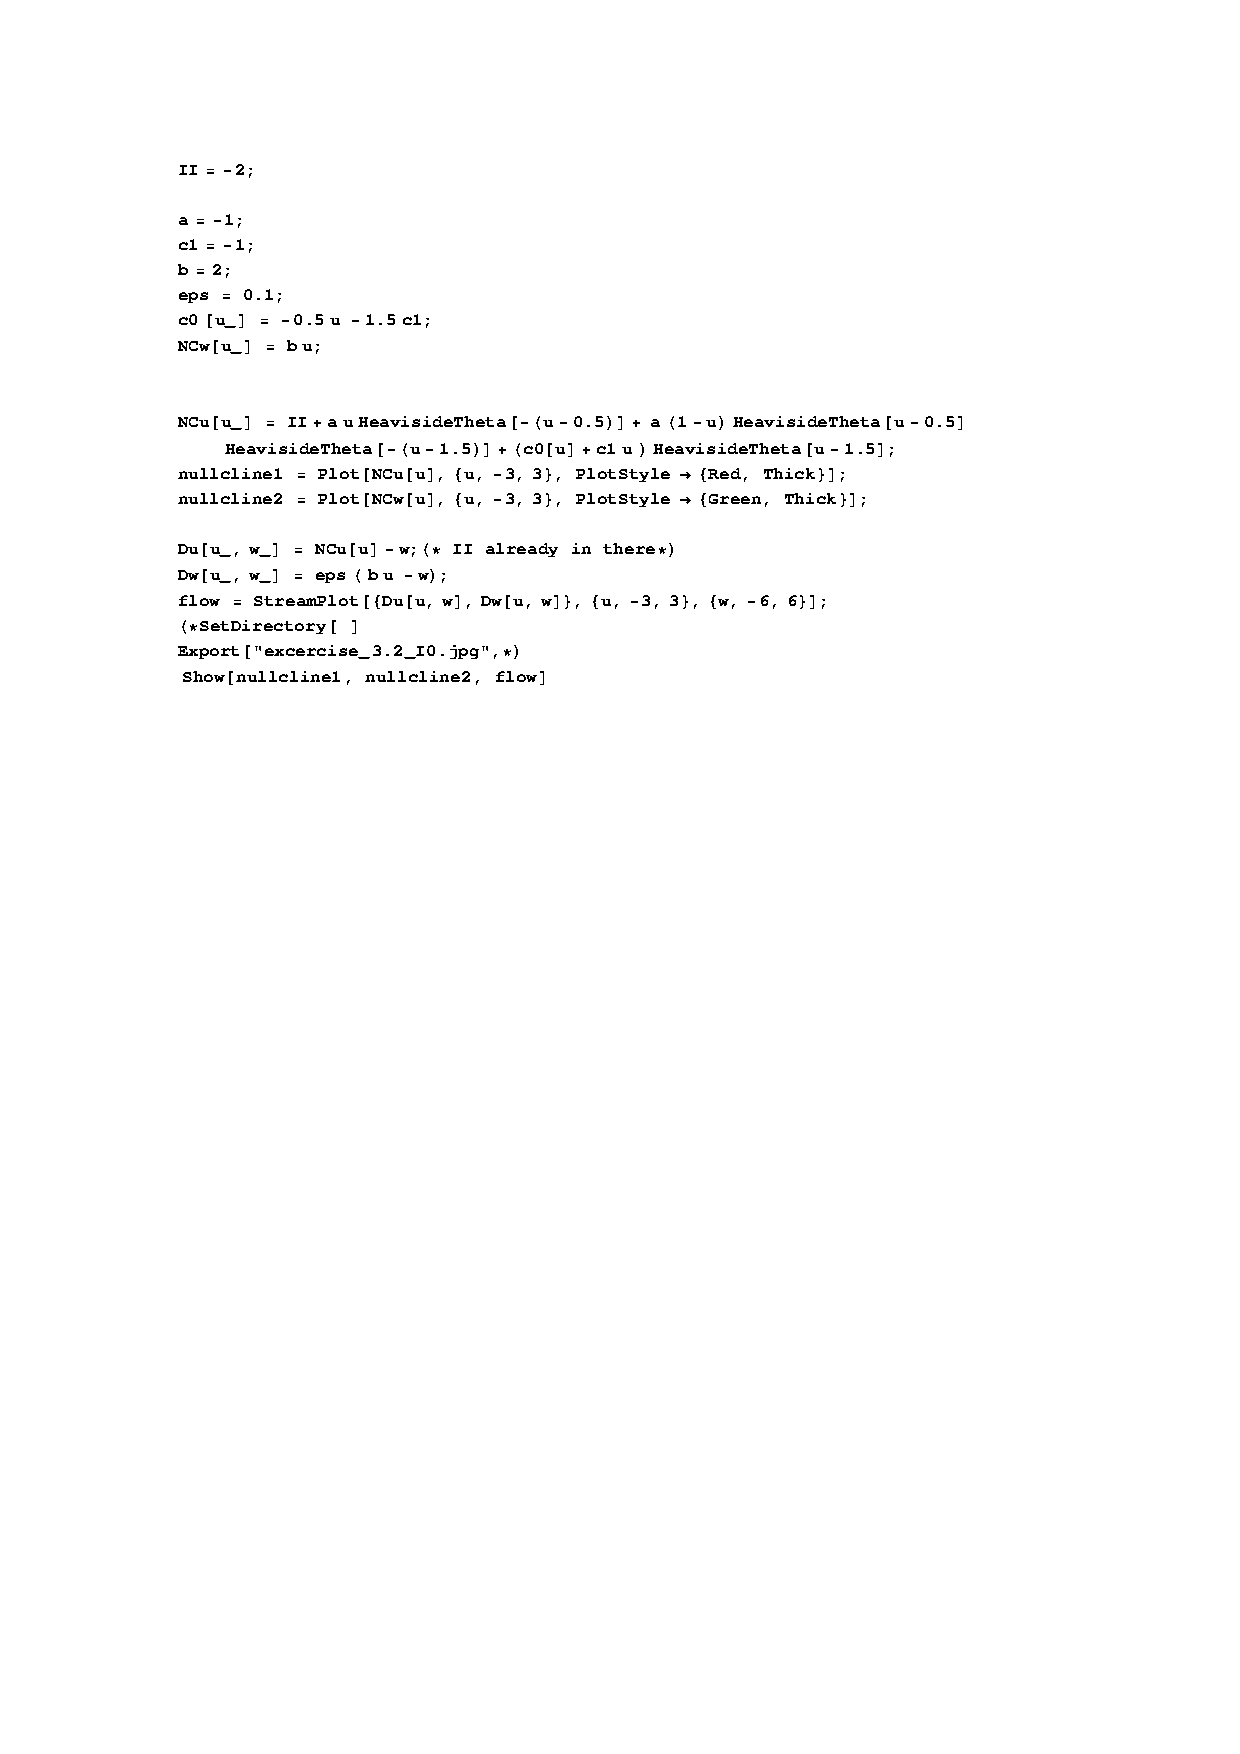
\includegraphics[width=5.2in]{code_32}

	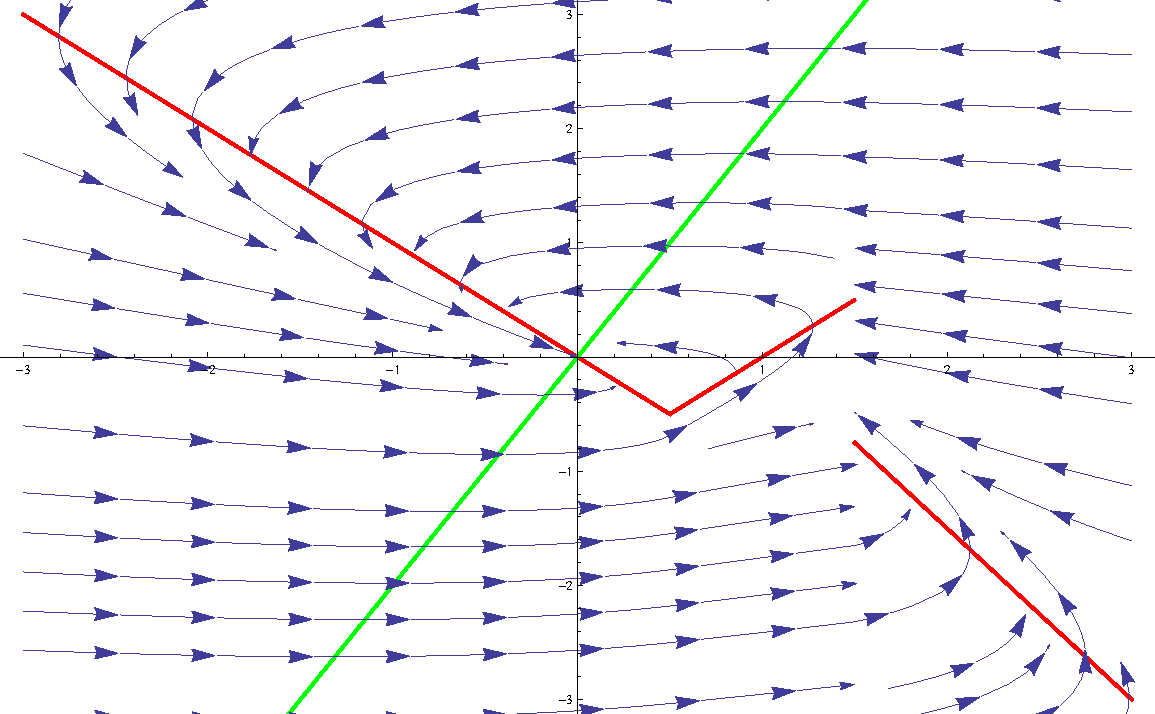
\includegraphics[width=5in]{excercise_32_I0}
\item Same as in a but with an input current of $I=-2$. The fixed point is calculated by the intersection of the following equations ($u<0.5$ compare figure):
	\begin{align}
		0 &= au - w -2 \\
		0 &= bu -w
	\end{align}
	which leads us to:
	\begin{align}
		u &= \frac{1}{a-b} = -\frac{2}{3} \\
		w &= au - 2 = -\frac{4}{3}
		\label{fixed}
	\end{align}
	the next figure shows the nullclines and the flow in the phase plane for $I=-2$

	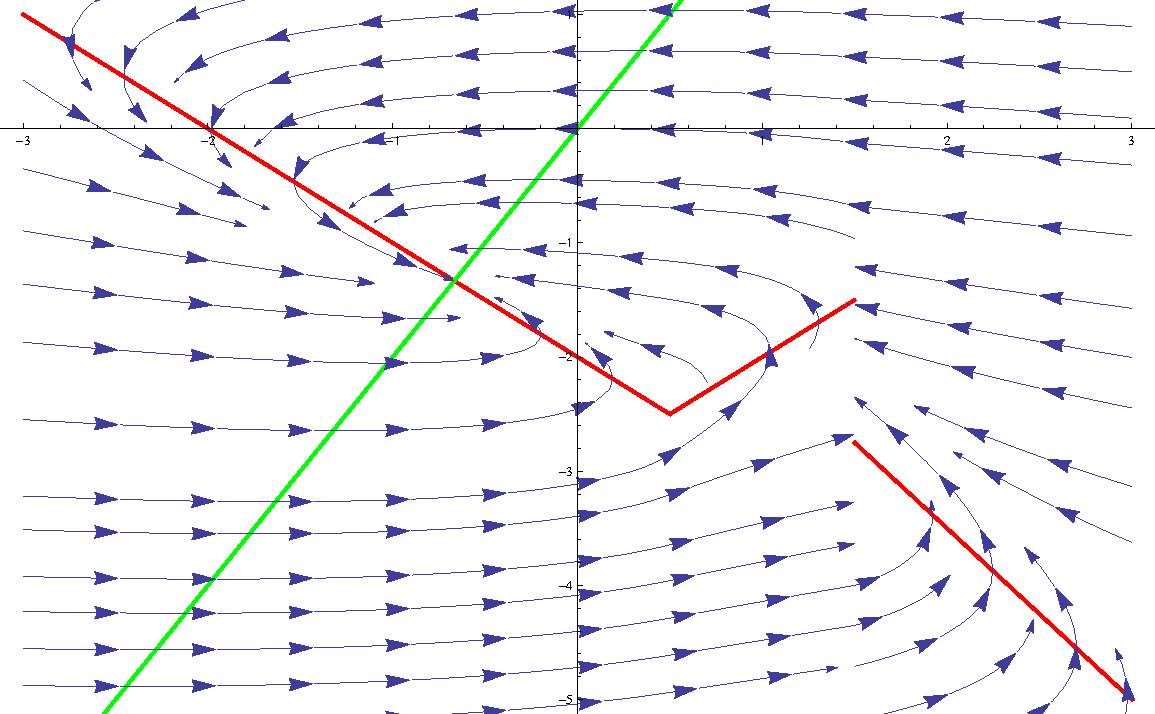
\includegraphics[width=5in]{excercise_32_I-2}
\item MATLAB code for simulation of the nullclines and trajectory in phase plane:
\begin{tiny}
\begin{lstlisting}
close all
clear all
clc

%%%%%%%%%%%%%%%%%%%%%%%%%%%
%% 0. PARAMETERS

% Euler integration
h = 10e-5;      % step size parameter
time = 500;     % simulation time

% Model
a = -1;
c1 = -1;
b = 2;
epsilon = 0.1;

t = 0:h:time; % generate time vector
I = [-1*(linspace(0,2,round(length(t)/2-1))) zeros(round(length(t)/2),1)']'; % create current vector

%%%%%%%%%%%%%%%%%%%%%%%%%%%
%% I. CALCULATE NULLCLINES

u = linspace(-3,3,length(t)); % preallocate voltage array
w = linspace(-3,3,length(t)); % preallocate w array
w = zeros(length(u),1); % preallocate aray for piecewise function

for i = 1:length(u)
    u1 = u(i);
    w(i) = fu(u1,a,c1);
end

nu = w + 0; % calculate voltage nullcline
nu_new = w - 2; % calculate voltage nullcline
nw = b*u; % calculate w nullcline
%%%%%%%%%%%%%%%%%%%%%%%%%%%
%% II. PERFORM INTEGRATION

u_sol = zeros(size(t)); % Preallocate array for velocities
w_sol = zeros(size(t)); % Preallocate array for positions

u_sol(1) = -2/3;%1.5;               % Initial condition gives solution for position at t=0.
w_sol(1) = -4/3;%0.375;             % Initial condition gives solution for velocity at t=0.

for i=1:(length(t)-1) % loop over time
    u_sol(i+1) = u_sol(i) + (fu(u_sol(i),a,c1) - w_sol(i) + I(i))*h; % integrate voltage DE
    w_sol(i+1) = w_sol(i) + epsilon*(b*u_sol(i) - w_sol(i))*h; % integrate w DE
end

%%%%%%%%%%%%%%%%%%%%%%%%%%%
%% III. PLOT REULTS
figure
hold on
grid on
plot(u,nu,'b','linewidth',2)
plot(u,nu_new,'k','linewidth',2)
plot(u,nw,'r','linewidth',2)
plot(u_sol,w_sol,'g','linewidth',2)
legend('u nullcline for I=0','u nullcline for I=-2','w nullcline','trajectory')
xlabel('u')
ylabel('w')
print(gcf,'-depsc','exercise32c_full.eps')
\end{lstlisting}
\end{tiny}

\begin{tiny}
\begin{lstlisting}
function f = fu(u,a,c1)
c0 = -0.5*u -1.5*c1;
if u<0.5
    f = a*u;
elseif 0.5 <= u && u < 1.5
    f = a*(1-u);
elseif u >= 1.5
    f = c0 + c1*u;
end
end
\end{lstlisting}
\end{tiny}

The next figure shows the trajectory in phase plane after the switch-off of the hyperpolarization current. The initial values for the Euler integration correspond to the calculated fixed point (Equation \ref{fixed})

\includegraphics[width=4.8in]{excercise32c_part}

The next figure shows the full trajectory in phase plane for a linearly increasing hyperpolarizing current, which is suddenly switched of. The initial values for the Euler integration are chosen to be $w=u=-2$. The $w$ nullcline is shown for $I=0$ and $I=-2$

\includegraphics[width=4.8in]{excercise32c_full}
\end{enumerate}

\end{exercise}

\begin{exercise}{3.3}
Exploring the FitzHugh model \\
\renewcommand{\labelenumi}{\alph{enumi})}
\begin{enumerate}
\item MATLAB code for Euler integration of FitzHugh-Nagumo model:
\begin{tiny}
\begin{lstlisting}
close all
clear all
clc

%%%%%%%%%%%%%%%%%%%%%%%%%%%
%% I. DEFINE PARAMETERs

% Euler
h = 10e-5; % step size parameter
time = 500; % simulation time
t = 0:h:time; % generate time vector

% model
epsilon = 0.1;
a = 15/8;
b = 3/2;
I = linspace(0,3,50); % create linear incresing current vector

rate = zeros(50,1); % preallocate rate array

for j = 1:length(I) % loop over currents
curr = I(j);
u = zeros(size(t)); % Preallocate array for velocities
w = zeros(size(t)); % Preallocate array for positions

u(1) = -1.5; % Initial condition gives solution for position at t=0.
w(1) = -0.375; % Initial condition gives solution for velocity at t=0.

numberOfPeaks = 0; % set counter
alreadyPeaked = 0; % set counter
threshold = 1; % set threshold

%%%%%%%%%%%%%%%%%%%%%%%%%%%%%%%%%%
%% II. PERFORM INTEGRATION
for i=1:(length(t)-1)
    u(i+1) = u(i) + (u(i) -u(i)^3/3 -w(i) + curr)*h; % integrate u
    w(i+1) = w(i) + epsilon*(a + b*u(i) - w(i))*h; % inegrate w
    % detection algorithm
    if(u(i+1) >= threshold)
        alreadyPeaked = 1;
    else
        if(alreadyPeaked == 1)
            alreadyPeaked = 0;
            numberOfPeaks = numberOfPeaks + 1;
        end
    end
end
rate(j) = numberOfPeaks/time; % normalize rate
end

%%%%%%%%%%%%%%%%%%%%%%%%%%%%%%%
%% III. PLOT RESULTS

figure                      % prepare figure
hold on                     % plot in every loop cycle in same figure
grid on                     % plot mesh grid
xlabel('Current')
ylabel('Rate')
plot(I,rate,'Linewidth',2)
print(gcf,'-depsc','ecxercise3ac.eps')
\end{lstlisting}
\end{tiny}
The next plot shows the firing rate as a function of input current

\includegraphics[width=4.4in]{excercise33a.eps} \label{currrate}
\item MATLAB code for calculating nullclines and an example trajectory
\begin{tiny}
\begin{lstlisting}
close all
clear all
clc

%%%%%%%%%%%%%%%%%%%%%%%%%%%%%
%% I. DEFINE PARAMETERS

% Euler integration
h = 10e-5; % step size parameter
time = 500; % simulation time
t = 0:h:time; % generate time vector

% model
a = 15/8;
b = 3/2;
epsilon = 0.1;
I = 2;

%%%%%%%%%%%%%%%%%%%%%%%%%%%%
%% II. CALCULATE NULLCLINES

u0 = linspace(-3,3,20000);

w1 = u0 - u0.^3/3 + I; % calculate u nullcline
w2 = a + b*u0; % calculate w nullcline

%%%%%%%%%%%%%%%%%%%%%%%%%%%
%% III. SOLVE DEs

u = zeros(size(t)); % Preallocate array for velocities
w = zeros(size(t)); % Preallocate array for positions

u(1) = -2; % Initial condition gives solution for position at t=0.
w(1) = -2; % Initial condition gives solution for velocity at t=0.

for i=1:(length(t)-1)
    u(i+1) = u(i) + (u(i) -u(i)^3/3 -w(i) + I)*h;
    w(i+1) = w(i) + epsilon*(a + b*u(i) - w(i))*h;
end

%%%%%%%%%%%%%%%%%%%%%%%%%%
%% IIII. PLOT RESULTS

figure
hold on
grid on
plot(u0,w1,'b','linewidth',2)
plot(u0,w2,'r','linewidth',2)
plot(u,w,'g','linewidth',2)
legend('u nullcline','w nullcline','trajectory')
xlabel('u')
ylabel('w')
print(gcf,'excercise33c_I2.pdf')
\end{lstlisting}
\end{tiny}

Plot of nullclines and trajectory at $I=0$ where $\nu=0$

	\includegraphics[width=4.0in]{excercise33c_I0.eps}

Plot of nullclines and trajectory at $I=2$ where $\nu\neq0$

	\includegraphics[width=4.0in]{excercise33c_I2.eps}
	\\\added{We interpret the plot as follows: in the first case the fixpoint in the phase space is reached fast, and the coordinates stay do not leave again. This means that the neuron adapts to the new state, i.e. the ion channels are opened until the equlibrium is reached. The current to which the cell was exposed is not large enough to induce spiking.}
	\\\added{On the contrary, for the second case no fixpoint is reached, the coordinates keep moving in the phase space. This behavior corresponds to a spiking trail, i.e. the used current was large enough for spiking. This is in agreement with the plot of the spiking frequency vs. the input current.}
\end{enumerate}

\end{exercise}

\end{document}